\section{FFOps\_\-Basic\_\-neu Class Reference}
\label{classFFOps__Basic__neu}\index{FFOps_Basic_neu@{FFOps\_\-Basic\_\-neu}}
Basic class for defining feed-forward neural networks. 


{\tt \#include $<$FFOps\_\-Basic\_\-neu.h$>$}

Inheritance diagram for FFOps\_\-Basic\_\-neu::\begin{figure}[H]
\begin{center}
\leavevmode
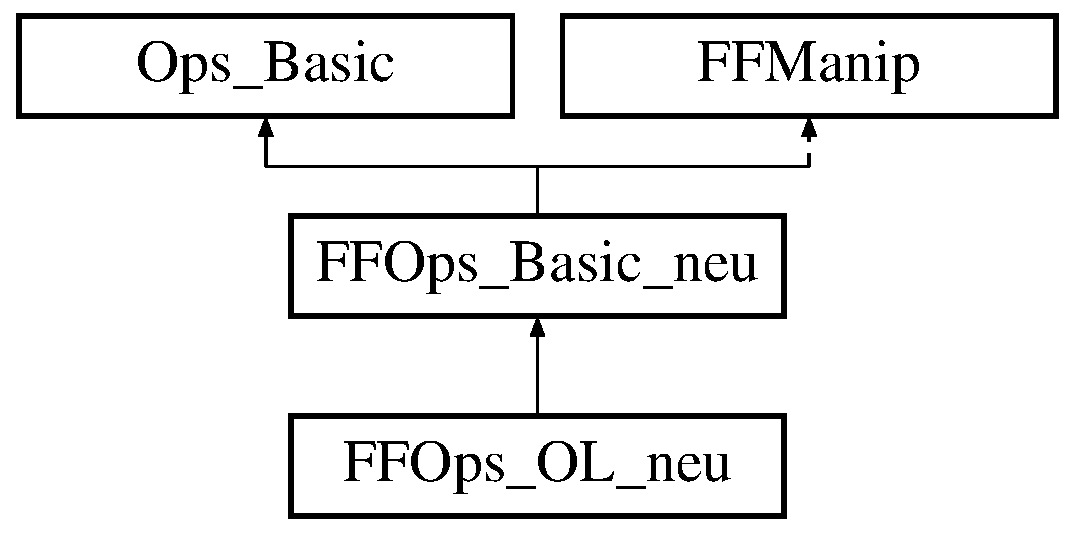
\includegraphics[height=3cm]{classFFOps__Basic__neu}
\end{center}
\end{figure}
\subsection*{Public Methods}
\begin{CompactItemize}
\item 
Individual {\bf create\-Empty} (const unsigned n\-In, const unsigned n\-Hidden, const unsigned n\-Out)
\begin{CompactList}\small\item\em This function creats a generic neural network.\item\end{CompactList}\item 
Array$<$ int $>$ {\bf get\-Connections\-Re\-Cla\-M} (Individual \&Ind)
\begin{CompactList}\small\item\em This function returns the connection matrix of the neural network.\item\end{CompactList}\item 
Array$<$ int $>$ {\bf get\-Connections\-Without\-Bias} (Individual \&Ind)
\begin{CompactList}\small\item\em This function also returns connection matrix of the neural network.\item\end{CompactList}\item 
Array$<$ double $>$ {\bf get\-Weights\-Re\-Cla\-M} (Individual \&Ind)
\begin{CompactList}\small\item\em This function returns the weigh value of the connections.\item\end{CompactList}\item 
void {\bf set\-Connections\-Re\-Cla\-M} (Individual \&Ind, Array$<$ int $>$ c\-R)
\begin{CompactList}\small\item\em This function defines the connections (structure) of a neural network.\item\end{CompactList}\item 
void {\bf set\-Weights\-Re\-Cla\-M} (Individual \&Ind, Array$<$ double $>$ c\-W)
\begin{CompactList}\small\item\em This function defines the weights of a neural network.\item\end{CompactList}\item 
void {\bf print\-Net} (Individual \&Ind, string filename)
\begin{CompactList}\small\item\em Print out the connections as well as the weights of the network.\item\end{CompactList}\item 
void {\bf print\-Net\-Without\-Bias} (Individual \&Ind, string filename)
\begin{CompactList}\small\item\em Print out the connections as well as the weights of the network.\item\end{CompactList}\item 
Array$<$ double $>$ {\bf get\-Gain} (Individual \&Ind)
\begin{CompactList}\small\item\em This function calculates the output of all neurons in the network.\item\end{CompactList}\item 
void {\bf set\-Activation} (Individual \&Ind, Array$<$ double $>$ activation)
\begin{CompactList}\small\item\em Set the activation value.\item\end{CompactList}\item 
Array$<$ double $>$ {\bf get\-Activation} (Individual \&Ind)
\begin{CompactList}\small\item\em This function returns the activation values of a network.\item\end{CompactList}\end{CompactItemize}


\subsection{Detailed Description}
Basic class for defining feed-forward neural networks.

This class defines feedforward neural networks based on the functions defined in {\tt Ops\_\-basic.h} and {\tt FFManip.h}. 



\subsection{Member Function Documentation}
\index{FFOps_Basic_neu@{FFOps\_\-Basic\_\-neu}!createEmpty@{createEmpty}}
\index{createEmpty@{createEmpty}!FFOps_Basic_neu@{FFOps\_\-Basic\_\-neu}}
\subsubsection{\setlength{\rightskip}{0pt plus 5cm}Individual FFOps\_\-Basic\_\-neu::create\-Empty (const unsigned {\em n\-In}, const unsigned {\em n\-Hidden}, const unsigned {\em n\-Out})}\label{classFFOps__Basic__neu_a0}


This function creats a generic neural network.

The neural network is generated given the number of input,  output and hidhen nodes. \begin{Desc}
\item[Parameters: ]\par
\begin{description}
\item[{\em 
n\-In:}]number of input nodes \item[{\em 
n\-Hidden:}]number of hidden nodes \item[{\em 
n\-Out:}]number of output nodes. \end{description}
\end{Desc}
\index{FFOps_Basic_neu@{FFOps\_\-Basic\_\-neu}!getActivation@{getActivation}}
\index{getActivation@{getActivation}!FFOps_Basic_neu@{FFOps\_\-Basic\_\-neu}}
\subsubsection{\setlength{\rightskip}{0pt plus 5cm}Array$<$double$>$ FFOps\_\-Basic\_\-neu::get\-Activation (Individual \& {\em Ind})}\label{classFFOps__Basic__neu_a10}


This function returns the activation values of a network.

\begin{Desc}
\item[Parameters: ]\par
\begin{description}
\item[{\em 
Ind:}]Individual representing the network to be accessed \end{description}
\end{Desc}
\index{FFOps_Basic_neu@{FFOps\_\-Basic\_\-neu}!getConnectionsReClaM@{getConnectionsReClaM}}
\index{getConnectionsReClaM@{getConnectionsReClaM}!FFOps_Basic_neu@{FFOps\_\-Basic\_\-neu}}
\subsubsection{\setlength{\rightskip}{0pt plus 5cm}Array$<$int$>$ FFOps\_\-Basic\_\-neu::get\-Connections\-Re\-Cla\-M (Individual \& {\em Ind})}\label{classFFOps__Basic__neu_a1}


This function returns the connection matrix of the neural network.

Notice that connections between the bias nodes are provided separately in column  at the end of the matrix. \begin{Desc}
\item[Parameters: ]\par
\begin{description}
\item[{\em 
Ind:}]Individual variable that defines the structure and parameters of the neural network. \end{description}
\end{Desc}
\index{FFOps_Basic_neu@{FFOps\_\-Basic\_\-neu}!getConnectionsWithoutBias@{getConnectionsWithoutBias}}
\index{getConnectionsWithoutBias@{getConnectionsWithoutBias}!FFOps_Basic_neu@{FFOps\_\-Basic\_\-neu}}
\subsubsection{\setlength{\rightskip}{0pt plus 5cm}Array$<$int$>$ FFOps\_\-Basic\_\-neu::get\-Connections\-Without\-Bias (Individual \& {\em Ind})}\label{classFFOps__Basic__neu_a2}


This function also returns connection matrix of the neural network.

However, the connection of the bias nodes are not included. \begin{Desc}
\item[Parameters: ]\par
\begin{description}
\item[{\em 
Ind:}]Individual variable that defines the structure and parameters of the neural network. \end{description}
\end{Desc}
\index{FFOps_Basic_neu@{FFOps\_\-Basic\_\-neu}!getGain@{getGain}}
\index{getGain@{getGain}!FFOps_Basic_neu@{FFOps\_\-Basic\_\-neu}}
\subsubsection{\setlength{\rightskip}{0pt plus 5cm}Array$<$double$>$ FFOps\_\-Basic\_\-neu::get\-Gain (Individual \& {\em Ind})}\label{classFFOps__Basic__neu_a8}


This function calculates the output of all neurons in the network.

\begin{Desc}
\item[Parameters: ]\par
\begin{description}
\item[{\em 
Ind:}]The network to be calculated defined by an individual \end{description}
\end{Desc}
\index{FFOps_Basic_neu@{FFOps\_\-Basic\_\-neu}!getWeightsReClaM@{getWeightsReClaM}}
\index{getWeightsReClaM@{getWeightsReClaM}!FFOps_Basic_neu@{FFOps\_\-Basic\_\-neu}}
\subsubsection{\setlength{\rightskip}{0pt plus 5cm}Array$<$double$>$ FFOps\_\-Basic\_\-neu::get\-Weights\-Re\-Cla\-M (Individual \& {\em Ind})}\label{classFFOps__Basic__neu_a3}


This function returns the weigh value of the connections.

The weights connecting the bias nodes are listed in column at the end of the matrix. \begin{Desc}
\item[Parameters: ]\par
\begin{description}
\item[{\em 
Ind:}]Individual variable that defines the structure and parameters of the neural network. \end{description}
\end{Desc}
\index{FFOps_Basic_neu@{FFOps\_\-Basic\_\-neu}!printNet@{printNet}}
\index{printNet@{printNet}!FFOps_Basic_neu@{FFOps\_\-Basic\_\-neu}}
\subsubsection{\setlength{\rightskip}{0pt plus 5cm}void FFOps\_\-Basic\_\-neu::print\-Net (Individual \& {\em Ind}, string {\em filename})}\label{classFFOps__Basic__neu_a6}


Print out the connections as well as the weights of the network.

The data are printed out to a file whose name is supplied by {\tt filename}. \begin{Desc}
\item[Parameters: ]\par
\begin{description}
\item[{\em 
Ind:}]The network to be printed out, which is represented by an individual. \item[{\em 
filename:}]name of the file to store the connections and weights of the network. \end{description}
\end{Desc}


Reimplemented from {\bf Ops\_\-Basic} {\rm (p.\,\pageref{classOps__Basic_a11})}.\index{FFOps_Basic_neu@{FFOps\_\-Basic\_\-neu}!printNetWithoutBias@{printNetWithoutBias}}
\index{printNetWithoutBias@{printNetWithoutBias}!FFOps_Basic_neu@{FFOps\_\-Basic\_\-neu}}
\subsubsection{\setlength{\rightskip}{0pt plus 5cm}void FFOps\_\-Basic\_\-neu::print\-Net\-Without\-Bias (Individual \& {\em Ind}, string {\em filename})}\label{classFFOps__Basic__neu_a7}


Print out the connections as well as the weights of the network.

The data are printed out to a file whose name is supplied by {\tt filename}. However, the biases are not included. \begin{Desc}
\item[Parameters: ]\par
\begin{description}
\item[{\em 
Ind:}]The network to be printed out, which is represented by an individual. \item[{\em 
filename:}]name of the file to store the connections and weights of the network. \end{description}
\end{Desc}
\index{FFOps_Basic_neu@{FFOps\_\-Basic\_\-neu}!setActivation@{setActivation}}
\index{setActivation@{setActivation}!FFOps_Basic_neu@{FFOps\_\-Basic\_\-neu}}
\subsubsection{\setlength{\rightskip}{0pt plus 5cm}void FFOps\_\-Basic\_\-neu::set\-Activation (Individual \& {\em Ind}, Array$<$ double $>$ {\em activation})}\label{classFFOps__Basic__neu_a9}


Set the activation value.

\begin{Desc}
\item[Parameters: ]\par
\begin{description}
\item[{\em 
Ind:}]Individual representing the network \item[{\em 
activation:}]a matrix that contains the activation values \end{description}
\end{Desc}
\index{FFOps_Basic_neu@{FFOps\_\-Basic\_\-neu}!setConnectionsReClaM@{setConnectionsReClaM}}
\index{setConnectionsReClaM@{setConnectionsReClaM}!FFOps_Basic_neu@{FFOps\_\-Basic\_\-neu}}
\subsubsection{\setlength{\rightskip}{0pt plus 5cm}void FFOps\_\-Basic\_\-neu::set\-Connections\-Re\-Cla\-M (Individual \& {\em Ind}, Array$<$ int $>$ {\em c\-R})}\label{classFFOps__Basic__neu_a4}


This function defines the connections (structure) of a neural network.

The network structure is defined by the connection matrix. \begin{Desc}
\item[Parameters: ]\par
\begin{description}
\item[{\em 
Ind:}]an individual representing a neural network \item[{\em 
c\-R:}]the connection matrix \end{description}
\end{Desc}
\index{FFOps_Basic_neu@{FFOps\_\-Basic\_\-neu}!setWeightsReClaM@{setWeightsReClaM}}
\index{setWeightsReClaM@{setWeightsReClaM}!FFOps_Basic_neu@{FFOps\_\-Basic\_\-neu}}
\subsubsection{\setlength{\rightskip}{0pt plus 5cm}void FFOps\_\-Basic\_\-neu::set\-Weights\-Re\-Cla\-M (Individual \& {\em Ind}, Array$<$ double $>$ {\em c\-W})}\label{classFFOps__Basic__neu_a5}


This function defines the weights of a neural network.

The network weights are given the connection matrix. \begin{Desc}
\item[Parameters: ]\par
\begin{description}
\item[{\em 
Ind:}]an individual representing a neural network \item[{\em 
c\-W:}]the weight matrix \end{description}
\end{Desc}


The documentation for this class was generated from the following file:\begin{CompactItemize}
\item 
FFOps\_\-Basic\_\-neu.h\end{CompactItemize}
